\documentclass{article} % For LaTeX2e
\usepackage{nips13submit_e,times}
%\usepackage{hyperref}
\usepackage{url}
\usepackage{graphicx}
%\documentstyle[nips13submit_09,times,art10]{article} % For LaTeX 2.09
%\usepackage{authblk}

\title{10-601B Group Project Final Report}

\author{
Liruoyang, Yu\\
MISM\\
\texttt{magicyuli@cmu.edu}
\and
Yilong, Chang\\
MISM\\
\texttt{yilongc@andrew.cmu.edu}
}


% The \author macro works with any number of authors. There are two commands
% used to separate the names and addresses of multiple authors: \And and \AND.
%
% Using \And between authors leaves it to \LaTeX{} to determine where to break
% the lines. Using \AND forces a linebreak at that point. So, if \LaTeX{}
% puts 3 of 4 authors names on the first line, and the last on the second
% line, try using \AND instead of \And before the third author name.

\newcommand{\fix}{\marginpar{FIX}}
\newcommand{\new}{\marginpar{NEW}}

%\nipsfinalcopy % Uncomment for camera-ready version

\begin{document}
\maketitle
\begin{abstract}
This report summarizes the final results of the 10-601B image classification group project. This report will conclude on the classifiers we implemented, the implementation methods, the experiments we did, and the comparison of the results.
\end{abstract}

\section{Introduction}
For the final submission, we trained and tested three classifiers, SVM,  Neural Network and k-NN. The dataset we used for training is a subset of 5000 images from CIFAR-10. We used VLFeat to extract HoG from images and then feed the extracted features to our classifiers.

We achieved 63\%, 62.7\% and 61.4\% accuracy on Autolab test using these three classifiers respectively.

\subsection{Motivation}

There are three reasons why we chose SVM. First is that image data is usually not linearly separable in the original feature space, and kernel SVM can deal with this kind of dataset pretty well. Second, the training of SVM is a convex optimization problem, which made it efficient to train. Third, SVM has relatively higher resistance to over-fitting because of the maximization of the margin. And it's easy to adjust C to avoid over-fitting.

We used Neural Network because it can learn very complicated patterns, especially when the net is deep (it's been proven that NN can simulate any function existing), so it fits our needs just right, since image classification is a very complicated.

We chose k-NN because it's extremely simple to implement and arrive at a good performance.

The classifiers we chose were all non-parametric because it's hard to assume a density distribution for the image features.

\subsection{Background and Related Work}
\subsubsection{Background}
"Image classification refers to the task of extracting information classes from a multiband raster image". And CIFAR-10 is an established dataset consisting of 60000 32$\times$32 color images in 10 classes used for the purpose of studying Image classification. 

\subsubsection{Related Work}

Kernel SVM has proven to be effective in the image classification field\cite{chapelle1999support} and was the go-to method before Convolutional Neural Network (CNN) exhibited its great power.

In recent years, CNN has been very successful in image classification. Some implementations of CNN have achieved state-of-the-art performance on the CIFAR-10 images, which are our target dataset. These works include a most recent model using fraction max-polling\cite{graham2014fractional}, reduced the error rate to 3.47\%. The Deeply Supervised Networks\cite{lee2014deeply}, by introducing a "companion" objective functions at each individual hidden layer they achieved an accuracy of 91.78\%. The Network in Network\cite{minlin2014network}, in which the authors built micro neural networks to abstract the data within the receptive field and obtained a 91.2\% accuracy.

\section{Method}

\subsection{Feature Engineering}

We used VLFeat to extract the Histogram of Oriented Gradient (HoG) of images, and use them as the features. HoG summarizes the magnitude of gradients along different directions at different positions of a image, which can reflect color and brightness changes.

\subsection{Data Preprocessing}
In order to prevent over-fitting and improve the training efficiency, we applied PCA to the extracted HoG data. Before PCA, there were 2304 feature dimensions. After PCA, we reserved the first 500 components for the Neural Network, which can explain 95\% of the variance, first 200 for SVM, which can explain more than 80\%, and first 143 for k-NN, which can explain approximately 74\%.

\subsection{Data Augmentation}
To prevent over-fitting and get more the training samples, we did data augmentation based on the 5,000 train samples. The method we used is to flip the images horizontally, and use the flipped images as the augmented set. So, in total, we trained our classifiers with 10,000 samples, 5,000 original, and 5,000 artificial.

\subsection{SVM}

\subsubsection{Training}

Since there are 10 classes of images, we adopted the 1 vs all strategy, i.e. training 10 classifiers based on the 10 labels we have.

We trained each classifier by maximizing the following dual problem of the objective function of SVM
\begin{equation}
W(\alpha)=\sum_{i=1}^{N}\alpha_{i}-\frac{1}{2}\sum_{i,j=1}^{N}\alpha_{i}\alpha_{j}y_{i}y_{j}K(\mathbf{x_{i}},\mathbf{x_{j}})
\end{equation}
\begin{equation}
0<\alpha_{i}<C
\end{equation}
,where $\mathbf{x_{i}}$ is the feature vector of a training sample after HoG and PCA, $y_{i}=1$ or $-1$ indicating whether $\mathbf{x_{i}}$ belongs to that class, $K(\mathbf{x_{i}},\mathbf{x_{j}})$ is the kernel trick.

Before the midway, we used the Gaussian Kernel as the kernel function
\begin{equation}
K(\mathbf{x_{1}},\mathbf{x_{2}})=e^{-\frac{||\mathbf{x_{1}}-\mathbf{x_{2}}||^{2}_{2}}{2\sigma^{2}}}
\end{equation}
However, afterwards, we found that for this dataset, the polynomial kernel performs better and greatly improves the computation efficiency compared to Gaussian kernel, so the kernel is computed as
\begin{equation}
K(\mathbf{x_{1}},\mathbf{x_{2}})=(\mathbf{x_{1}}\cdot\mathbf{x_{2}})^3
\end{equation}

We used quadprog() in Matlab to find the $\mathbf{\alpha}$ that maximizes function (1), then compute the bias as
\begin{equation}
b=\frac{\sum_{i=1}^{N}\alpha_{i}y_{i}}{\#~of~\alpha_{i}\neq{0}}
\end{equation}

\subsubsection{Predicting}

We predicted the class $c$ for new samples based on
\begin{equation}
c=\arg\max_{c}\sum_{i=1}^{N}\alpha_{i,c}y_{i,c}K(\mathbf{x_{i}},\mathbf{x_{new}})+b_{c}
\end{equation}

\subsection{Neural Network}
In this phase, we first implemented batch mode. Then we upgraded our basic model to a two-hidden-layered Network and compared the performance with the basic one. The boost of adding a layer was not remarkable, but the result proved incremental mode gradient descent was better. After we tested several layer numbers, we decided to use a Network with three hidden layers. Since we used 500 features, the number of input nodes was 500. And the number of nodes for the hidden layers were 150, 150, 100 respectively.

\subsubsection{Training}
During the training process, we used Rectified Linear Units for all the nodes in the hidden layers, whose activation function is as follow:
\begin{equation}
a_{i}^{l}=max(0,z_{i}^{l})
\end{equation}
where
\begin{equation}
z_{i}^{l}=\sum_{k=1}^{K_{l-1}}w_{ik}^{l}a_k^{l-1}+b_{i}^{l}
\end{equation}
where $K_{l-1}$ is the number of nodes in layer $l-1$, $w_{ik}^{l}$ is the weight from the node $k$ in layer $l-1$ to node $i$ in layer $l$, $a_k^{l-1}$ is the activation of node $k$ in layer $l-1$, and $b_{i}^{l}$ is the bias for node $i$ in layer $l$.

And for the output layer, we used softmax as the activation function:
\begin{equation}
p(c_k=1|x) =  \frac{e^{o_k}}{\sum_{j=1}^{C}e^{o_j}}
\end{equation}
where $o_{j}$ is the output for class j, and $o_{j}$ is in range of (0, 1) adding up to 1. C is the number of classes. 

The loss function we used is the negative log-likelihood function:
\begin{equation}
L(x, y; \theta) = -\sum_jy_j\log p(c_j|x)
\end{equation}

The learning process is minimizing the loss over the whole training set:
\begin{equation}
\theta^* = \arg\min_\theta\sum_{n=1}^NL(x^n, y^n; \theta)
\end{equation}
where N is total number of samples in training set. 

To diminish the fluctuations in weight changes over consecutive iterations and prevent over-shotting, we incorporated momentum into stochastic gradient descent weight update as follows:
\begin{equation}
\Delta \leftarrow \mu\Delta-\eta\frac{\partial L}{\partial \theta}
\end{equation}
\begin{equation}
\mathbf{\theta} \leftarrow \mathbf{\theta}+\Delta
\end{equation}
where $\Delta$ is the momentum, $\mu$ is the fraction coefficient (we set as 0.9), $\eta$ is the learning rate, $L$ is the loss function, and $\theta$ is the model parameters.

And we adopted early stop strategy to prevent over-fitting, where we stopped the training based on the number of epochs.

\subsubsection{Predicting}
We predicted the class of test data with forward propagation as:
\begin{equation}
\hat{y}=\arg\max_{c}o_{c}
\end{equation}
where $o_{c}$ is the output of the nodes in the output layer for class c.

\subsection{k-NN}
\subsubsection{Training}
The training process for k-NN is just augment the dataset and save the model.
\subsubsection{Predicting}
To predict the labels using k-NN, we first compute the similarity between a test sample $x_{test}$ and all other training samples $x_{i}$, and let the k samples that are most similar to $x_{test}$ vote using their similarities, and predict the label which has the most votes. Formally, the labels are determined by
\begin{equation}
v_{c}=\sum_{y_{i}=c}sim(\mathbf{x_{i}},\mathbf{x_{test}})
\end{equation}
\begin{equation}
\hat{c}=\arg\max_{c}v_{c}
\end{equation}
where $v_{c}$ is the vote for class $c$, $sim(\mathbf{x_{i}},\mathbf{x_{test}})$ is the dot product similarity between $\mathbf{x_{i}}$ and $\mathbf{x_{test}}$, and $\hat{c}$ is the predicted label.
\subsection{Evaluation}

We evaluated our classifier by accuracy on the validation set and the test set on Autolab. And when training Neutral Network, we evaluated the model we trained by the negative log-likelihood loss on the training set.

We also leveraged validation to select the optimal hyper-parameters as described in section \ref{experiments}, Experiments and Results.
\section{Experiments and results}
\label{experiments}

\subsection{SVM}

\subsubsection{Linear SVM vs Kernel SVM}
Before the midway, we experimented with both Linear SVM and Kernel SVM, and it turned out that Linear SVM achieved best accuracy of 53\% on the validation set, whereas Kernel SVM achieved 61.8\%.

\subsubsection{Gaussian Kernel vs Polynomial Kernel}
After midway, we experimented with polynomial kernel function, and it gives the same classification performance, but improves the calculation efficiency by a great amount. So, we used polynomial kernel function afterwards.

\subsubsection{Hyper-parameter Selection}

There are two hyper-parameters for Gaussian Kernel SVM, namely $C$ and $\sigma$. We selected these hyper-parameters by validation. We separated the 5,000 samples in the training set into one training set of 4,000 samples and one validation set of 1,000 samples.

We selected $\sigma$ and $C$ based on the accuracy on the validation set. 

Before the midway, the $\sigma$ and $C$ we selected were 1.9 and 100, which achieved 61.8\% accuracy on the validation set. And since we used different kernel function and different number of principle components  after that, we change $C$ to 0.0022, and eliminated $\sigma$, which gave us validation set accuracy of 64\%.

\subsubsection{Autolab Submission}
Our Polynomial Kernel SVM classifier achieved 63\% accuracy on Autolab test set.


\subsection{Neural Network}
Besides the models we introduced in the mid-way report, we tried other techniques and regularization terms. In both training processes we first initialized the weights vectors $\mathbf{w_i}$, which was the weight vector between input layer and the first hidden layer and also between hidden layers, and $\mathbf{u}$, the weight vector between the last hidden layer and output layer with random number $\sim$ $N$(0, $N$), where $N$ is the size of training set. The next few subsections deal with both the models in the last phase and the new optimization we tried.
\subsubsection{Basic Neural Network}
In the first model, we set a fixed learning rate at:
\begin{equation}
\eta = 2
\end{equation}
We used the 4000 samples to train. Once the change rate of RMSE was less than 0.0005, we would stop the iteration.

The highest accuracy on local machine was 54.1\%. We submitted a model of 52.8\% on Autolab and the result was 48.4\%. 

\subsubsection{Regularized Neural Network}
In the second model, we added two bias vectors $\mathbf{b1}$ and  $\mathbf{b2}$ with initial values from [-0.5, 0.5], and updated these two vectors together with weight vectors.

This time, we set the learning rate at:
\begin{equation}
\eta = \frac{2}{\sqrt{m}},
\end{equation}
where m is the current number of epoch. 

To avoid over-fitting, we regularized using Simple Weight Decay:
\begin{equation}
\mathbf{w}\rightarrow\mathbf{w_0}-\frac{\eta\lambda}{n}
\end{equation}
where $\mathbf{w_0}$ is the weight vector before regularization.

After some trials, we set the parameters and trained the model with all the 5000 samples.

The accuracy on training data before regularization was around 90\%, but decreased to around 78\% after regularization. And the test result on Autolab was 50\%.

\subsubsection{Autolab Submission}
Our basic NN with Regularization achieved 50\% accuracy on Autolab.

\subsection{A somewhat Deep Neural Network}
To arrive at the final NN we used, we did following experimentations.

\subsubsection{Number of Hidden Layers}
Before midway, our 3-layer NN could only achieve test accuracy around 50\%. So, in order to discover more sophisticated patterns in the feature and improve the performance, we decided to add more hidden layers. It turned out that it worked, the 5-layer NN gave us 62.7\% accuracy on the test set. However, we found more layers wouldn't improve the performance further because of over-fitting.

\subsubsection{Activation and Lost Functions}
When initially adding extra hidden layers, the accuracy didn't get improved, and the reason was after the NN got deeper, due to gradient vanishing, the gradients with sigmoid function for the front layers diminished very fast as the error back-propagates. So, the hidden layers became hard to train.

To solve this, we experimented other activation functions and loss functions, namely the ReLU and softmax activation functions, and Cross-Entropy and Negative Log-Likelihood loss functions. These experiments sped up the training process by great amount, due to the mathematical properties of these functions. Only after this, our 5-layer NN got trained properly.

\subsubsection{Weight Initialization}
We initialized the weights for each layer based on the empirical rule\cite{cs231ninit}, sampling from normal distributions with $\mu=0$ and $\sigma=\frac{1}{\sqrt{\# nodes~in~the~previous~layer}}$.

The adoption of this strategy greatly improved the learning speed of our NN, compared to when we set $\sigma=\frac{1}{\sqrt{\# training samples}}$ for the normal distributions we sampled from, because this makes the initial activations of every layer have similar deviations.

\subsubsection{Learning Rate}
First we tried to diminish by the mini-batch iterations, and we found that it often rendered the training to be trapped in local-minimums. So, in order to explore wider solution space, we chose not to diminish the learning rate, while set it to be a smaller value, e.g. 0.01.

We also tried self-adjusted learning rate and momentum, e.g. AdaGrad, but it didn't work out.

\subsubsection{Number of Training Epochs}
We also experimented with the number of epochs for early stop. We chose the number of epochs to be 289 based on the validation results shown in \figurename{1}.
\begin{figure}[ht!]
	\centering
	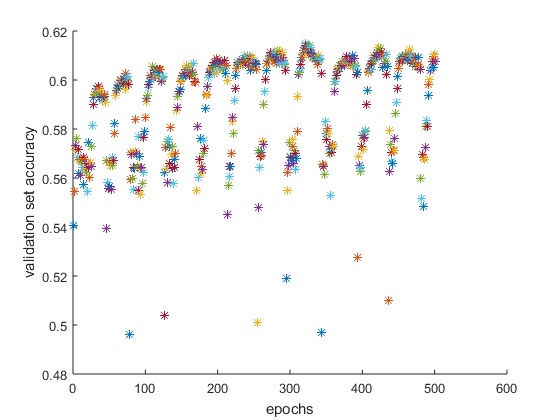
\includegraphics[width=90mm]{dnn_train_500.png}
	\caption{Validation set accuracy under different training epochs}
\end{figure}

\subsubsection{Autolab Submission}
Our 5-layer NN with Regularization achieved 62.7\% accuracy on Autolab.


\subsection{K Nearest Neighbors}

\subsubsection{K}
$K$ is the most important hyper-parameter for k-NN. We experimented with different values of $K$. We determined $K$ by validation. As shown in \figurename{2}, we chose $K$ to be 233.
\begin{figure}[ht!]
	\centering
	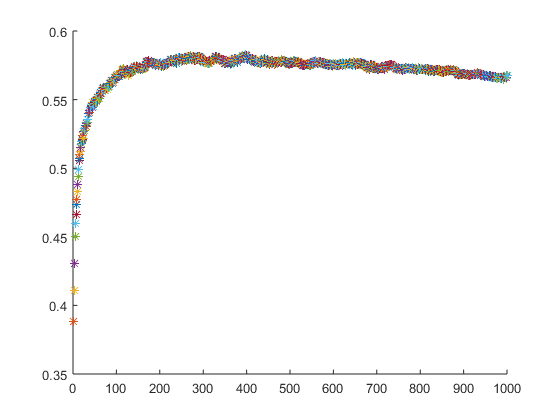
\includegraphics[width=90mm]{knn.png}
	\caption{Validation set accuracy under different K}
\end{figure}

\subsubsection{Autolab Submission}
Our k-NN achieved 61.4\% accuracy on Autolab.

\subsection{Multi-class Boosting}
In addition to the experiments above, we also tried multi-class boosting using Logistic Regression. But it turned out to need too many training iterations to have a good performance, we finally changed to k-NN.


\section{Conclusion}
From this project, we closely got in touch with SVM and Neural Network, and we did a lot of tunings and experiments on them to achieve the results. In comparison, k-NN was rather straightforward and simple, and we were surprised by its good performance.

Although we didn't get exceptional accuracy for SVM and NN, but we definitely saw the power they can exhibit in the area of image classification. Based on our experience, we think if we were to further improve the accuracy, we either need more sophisticated feature extraction techniques (we found that HoG doesn't work well when the objects to be detected are not in the center of the images or have various sizes), or to use a classifier such as CNN, which can automatically detect the features on the images, no matter where the objects are or what the sizes they are. We think this is why CNN has such a incompatible performance on image classification.



\bibliographystyle{abbrv}
\bibliography{nips2013}  % sigproc.bib is the name of the Bibliography
\end{document}
